\begin{flushright} {\tiny {\color{gray} python\_codes/fieldstone\_01/text.tex}} \end{flushright}

\lstinputlisting[language=bash,basicstyle=\small]{python_codes/fieldstone_01/keywords}

\begin{center}

\fbox{\textbf{\huge \color{teal} P}}
\fbox{\textbf{\huge \color{purple} J}}
\fbox{\textbf{\huge \color{orange} F}}
Codes at \url{https://github.com/cedrict/fieldstone/tree/master/python_codes/fieldstone_01}
\end{center}

\par\noindent\rule{\textwidth}{0.4pt}

{\sl This fieldstone was developed in collaboration with Job Mos}. \index{contributors}{J. Mos}

\par\noindent\rule{\textwidth}{0.4pt}
%%%%%%%%%%%%%%%%%%%%%%%%%%%%%%%%%%%%%%%%%%%%%%%%%%%%%%%%%%%%%%%%%%%%%%%%%%%%%%%%%%%%%%%%%%%%%%

This benchmark is taken from Donea \& Huerta (2003) \cite{dohu03} and is described fully in section \ref{mms1}. 
In order to illustrate the behavior of selected mixed finite elements in the solution 
of stationary Stokes flow,  we consider a two-dimensional problem 
in the square domain $\Omega=[0,1]\times[0,1]$, which possesses a closed-form analytical 
solution. 

\begin{center}
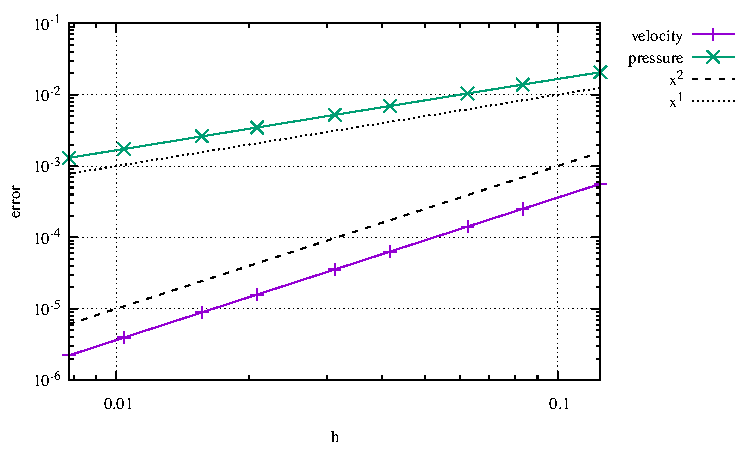
\includegraphics[width=10cm]{python_codes/fieldstone_01/results/errors.pdf}\\
{\captionfont Quadratic convergence for velocity error, 
linear convergence for pressure error, as expected.}
\end{center}

\begin{center}
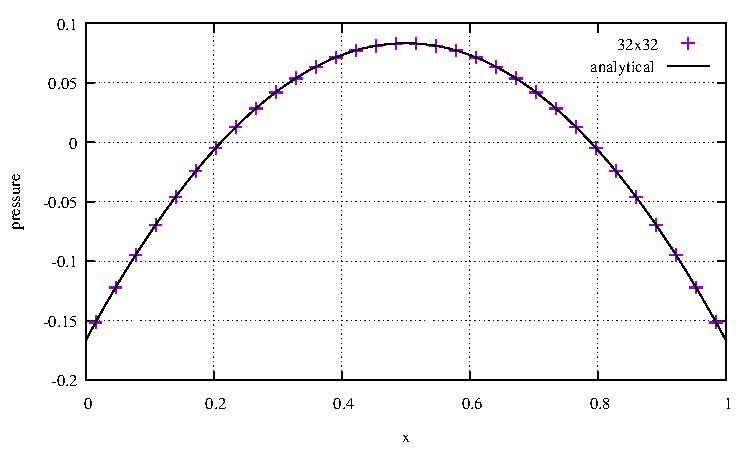
\includegraphics[width=10cm]{python_codes/fieldstone_01/results/pressure.pdf}\\
{\captionfont Pressure field}
\end{center}

\begin{center}
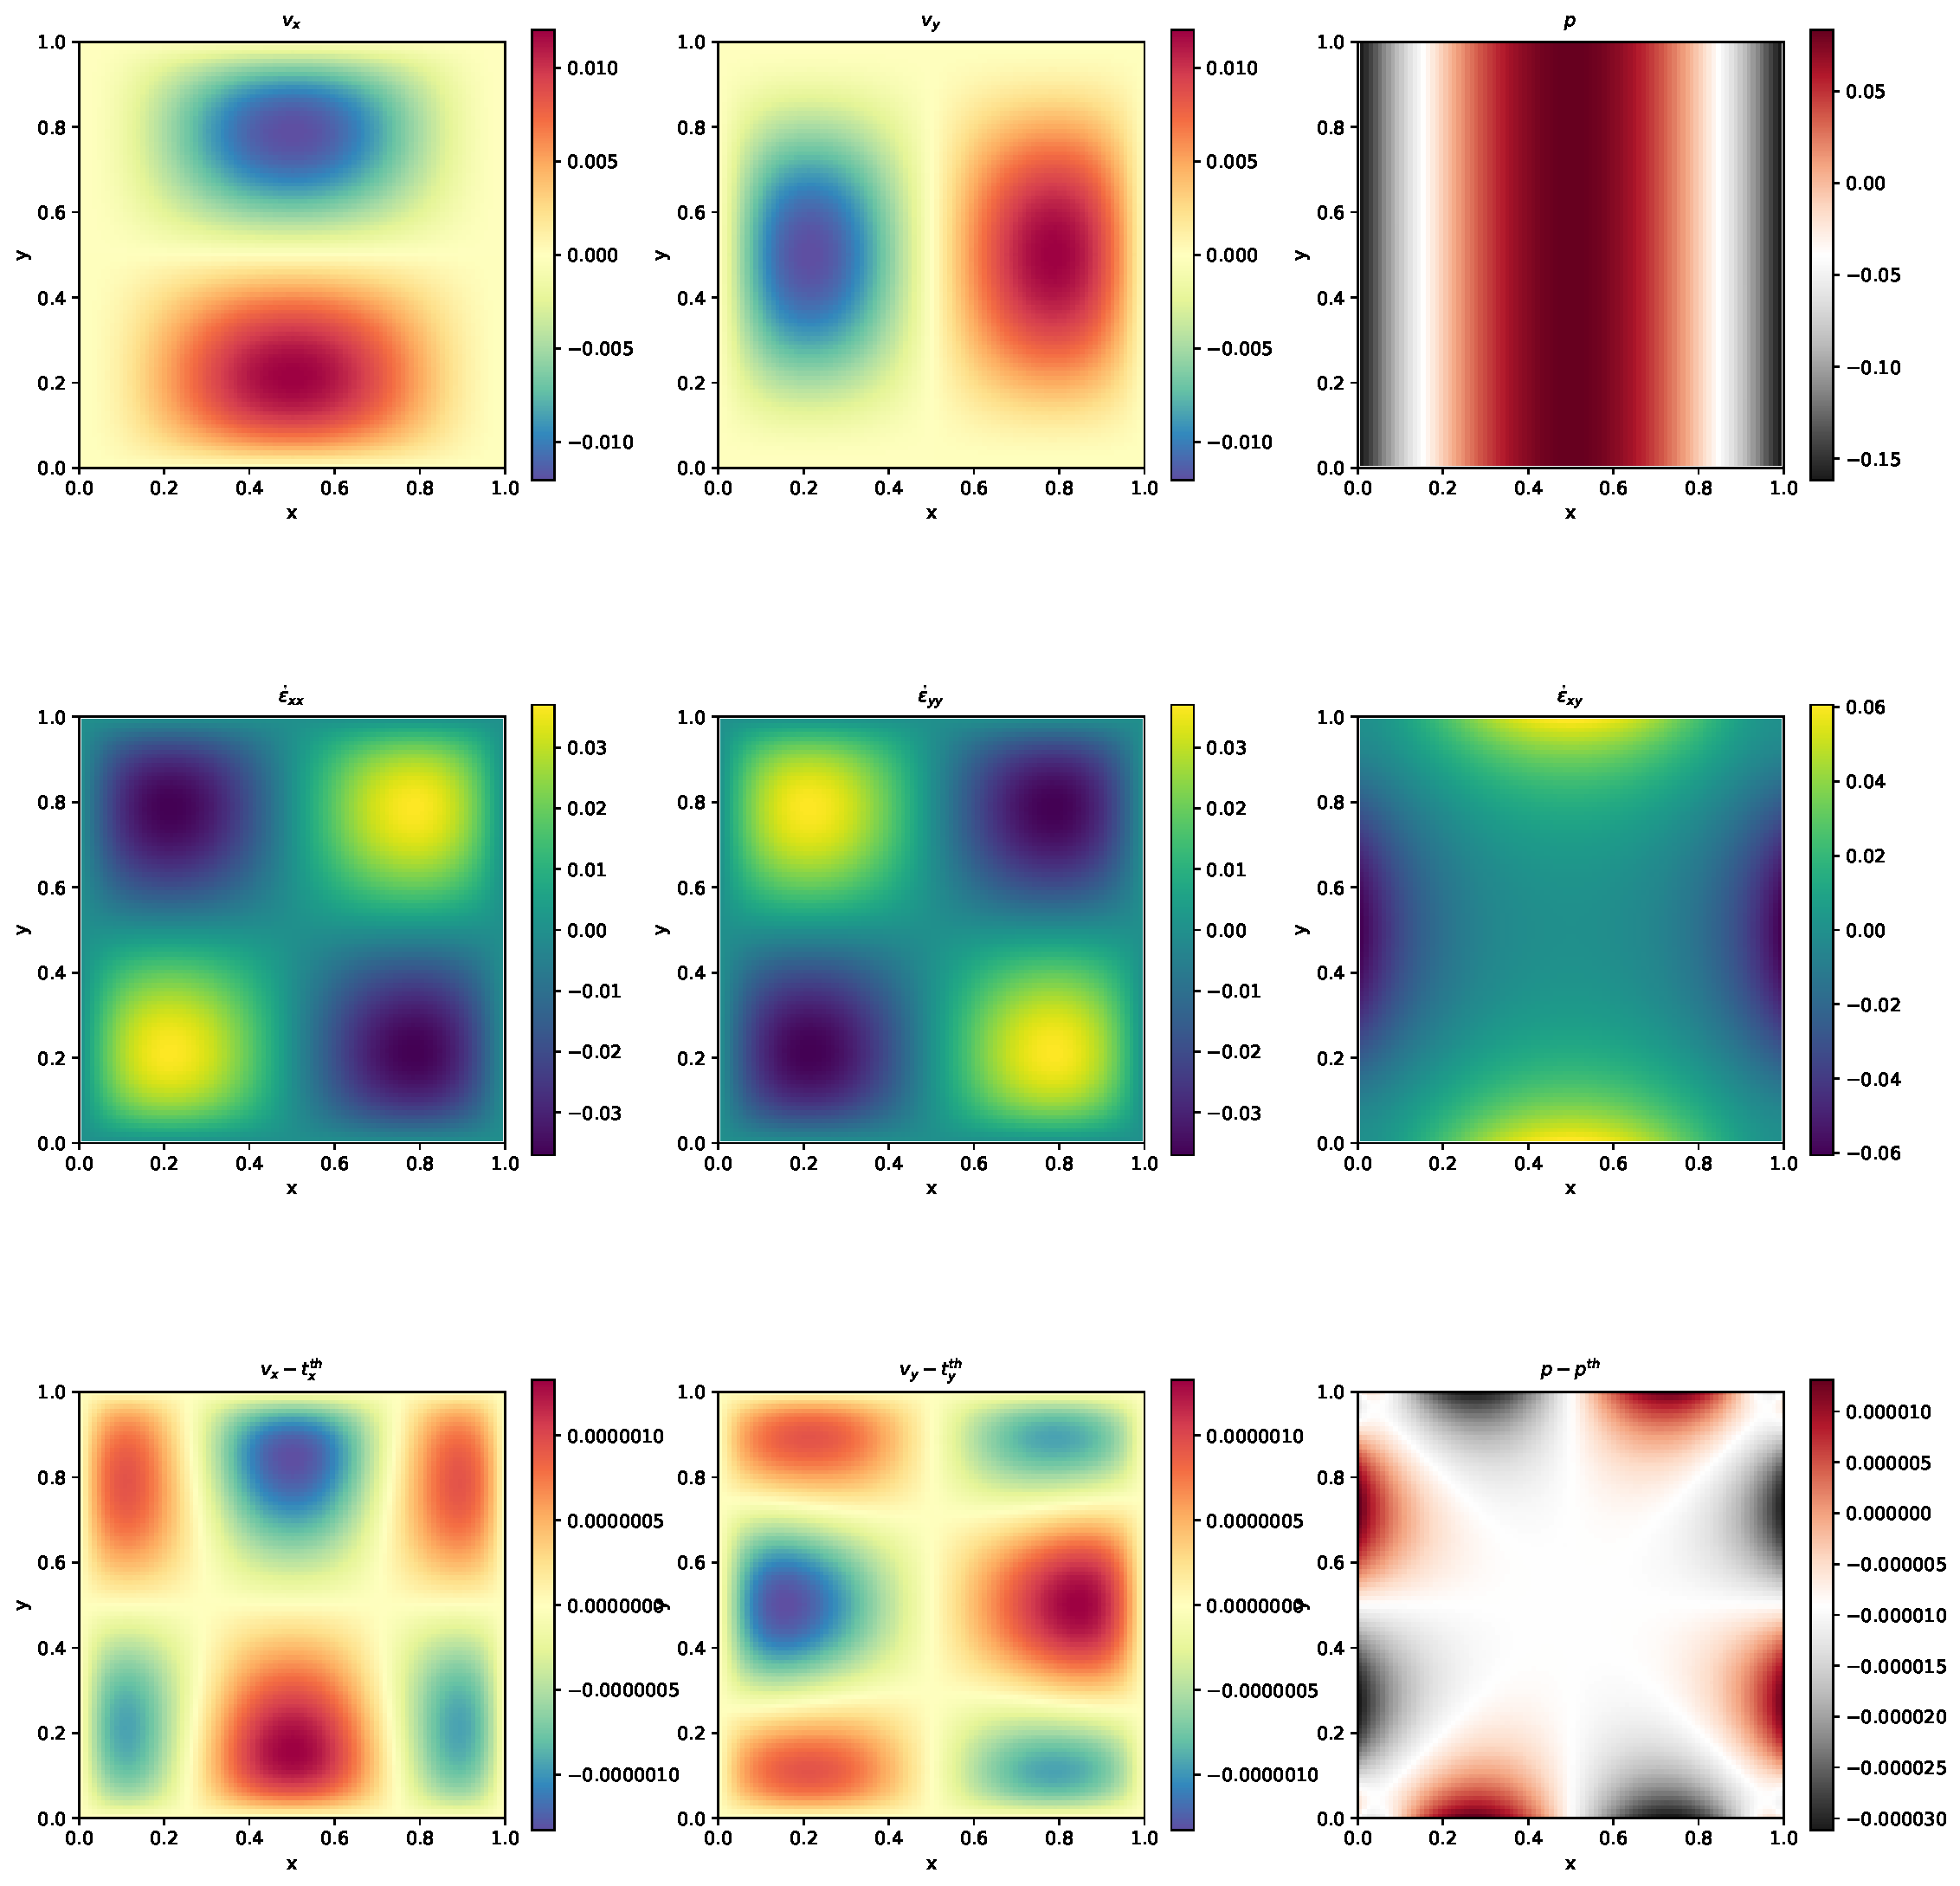
\includegraphics[width=15cm]{python_codes/fieldstone_01/solution.pdf}
\end{center}

One can also compute vertical/depth averages of the velocity, see Eq.~\eqref{eq:dhvelnorm}.
Note that the averages are computed somewhat naively: instead of computing integrals in the $x$-direction
at many depths I simply take an arithmetic average over rows of nodes. At high resolution the profiles
converge to the analytical profiles for the individual components and to the results 
obtained with \aspect. Please check \stone~110 for a better implementation.
\begin{center}
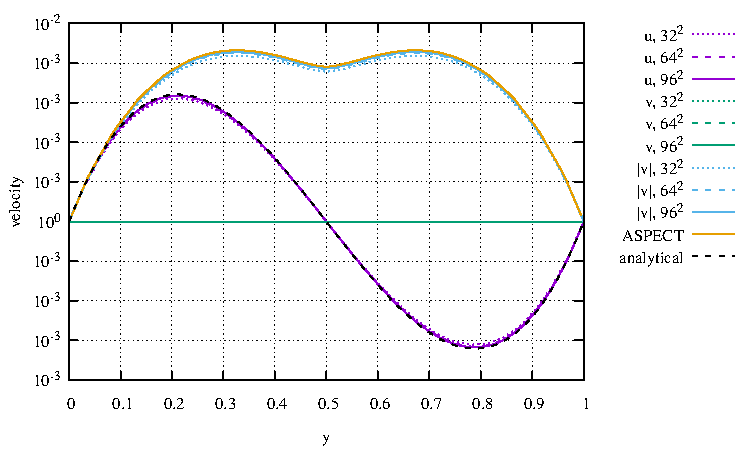
\includegraphics[width=10cm]{python_codes/fieldstone_01/results/vel_profile}\\
{\captionfont Vertical average of velocity. \aspect was run with the 'depth average' postprocessor
added to the prm file.}
\end{center}

\newpage
\subsection*{About the Fortran code}

I wrote the first ever version of this \stone in
Fortran90 around 2011. It is available in the {\foldernamefont simplefem} folder in this stone.
\index{general}{fortran90}

The code can be compiled as follows:
\begin{verbatim}
> gfortran -O3 linpack_d.f90 blas_routines.f simplefem.f90
\end{verbatim}
and run as follows:
\begin{verbatim}
> ./a.out 
\end{verbatim}
The solver used here does not make use of a sparse storage and relies on a dense matrix 
set of subroutine from BLAS and LinPACK\footnote{\url{https://en.wikipedia.org/wiki/LINPACK}}.
\begin{center}
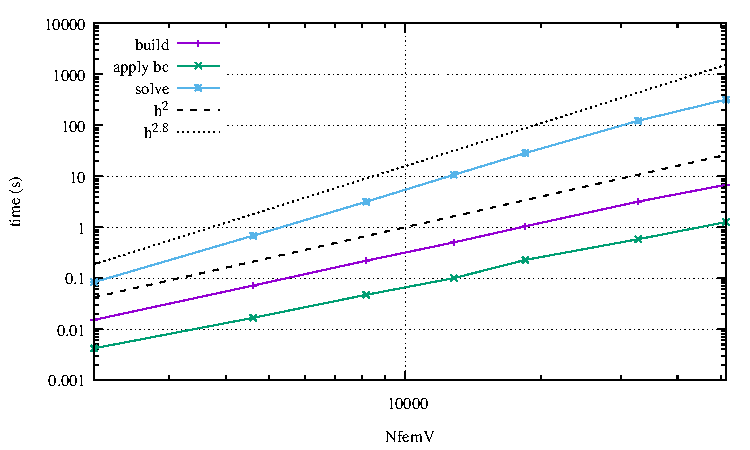
\includegraphics[width=9cm]{python_codes/fieldstone_01/simplefem/timings/timings.pdf}\\
{\captionfont Despite a very naive application of the boundary conditions to the entire
assembled FE matrix, we find here that this part of the code is not taking long at all.}
\end{center}
There is no export of the results to ParaView format, only ascii text files.



\newpage
\subsection*{About the Julia code}









